\section{검증 및 실험 평가}
\label{sec:evaluation}

이 절은 프로토콜 구성과 조건부 분석을 보완하여 두 가지를 확인한다.
첫째, 기록을 따라가고 남은 대상을 차단하는 동작이 맞는가.
둘째, 거래와 감사에 얼마나 많은 계산·원장 작업·시간이 필요한가.
먼저 측정 방법을 설명하고, 동작과 비용의 결과를 제시한 뒤
기존 연구와 비교할 수 있는 범위를 정리한다.

\subsection{실험 환경 및 방법}

Table~\ref{tab:evidence-scope}는 보안 분석과 평가 근거의 역할을
구분한다. 기호 모델은 정해진 사례의 논리 동작을, 시제품 실행은
대표 경로의 연결을, 성능 자료는 선택한 조건의 비용을 보여 준다.
이들은 동일한 판본을 사용한 하나의 통합 검증 결과가 아니다.

\begin{table}[ht]
\centering\small
\caption{Scope of the analysis and evaluation evidence}
\label{tab:evidence-scope}
\begin{tabularx}{\columnwidth}{@{}>{\raggedright\arraybackslash}p{.19\columnwidth}Y@{}}
\toprule
Evidence & Supported result and boundary \\ \midrule
Proofs & Conditional correctness, soundness, and passive privacy; no concrete conformance result. \\
Symbolic model & Selected accounting, tracing, and completion cases; no cryptographic execution or full specification validation. \\
Prototype & Selected paths at \texttt{8560fd3}; test verifier and single audit-key version. \\
Costs & Measured workload costs; independent-run variability and some version/configuration mappings remain unresolved. \\
\bottomrule
\end{tabularx}
\end{table}

성능 측정 환경은 Table~\ref{tab:eval-env}와 같다.
회로는 PLONK-KZG와 BLS12-381을 사용하고, 감사 암호화에는
Jubjub와 Poseidon2를 사용한다. 원장 실행 환경은 로컬 Anvil이다.
기호 검사, 고정된 시제품 판본의 실행 기록과 성능 측정 자료는
평가 아티팩트에 정리되어 있다~\cite{zkdpp-evaluation-artifact-2026}.

\begin{table}[ht]
\centering\small
\caption{Performance measurement environment}
\label{tab:eval-env}
\begin{tabularx}{\columnwidth}{@{}lY@{}}
\toprule
Item & Configuration \\ \midrule
Host & MacBook Pro (MacBookPro18,1) \\
OS & macOS 26.3 (25D125) \\
CPU & Apple M1 Pro, 10 cores (8 performance + 2 efficiency) \\
Memory & 32 GB \\
Circuit libraries & gnark 0.15.0; gnark-crypto 0.20.1 \\
Proof / curve & PLONK-KZG / BLS12-381 \\
Audit curve / hash & Jubjub / Poseidon2 \\
Ledger node & Anvil 1.7.1 \\
Compiler / EVM & Solidity 0.8.30 / Prague \\
\bottomrule
\end{tabularx}

\end{table}


비용은 세 지표로 본다. \emph{제약 수}는 증명 회로에 표현한
계산 조건의 수다. \emph{gas}는 원장이 거래를 처리할 때 수행한
작업량을 나타내는 단위로, 지불 금액 자체는 아니다.
성공한 거래 영수증의 \texttt{gasUsed} 값을 사용한다.
\emph{전체 실행 시간}(E2E)은 비공개 입력을 준비하기 시작한 때부터
거래가 성공했다는 영수증을 확인할 때까지의 시간이다.
세 지표가 측정하는 작업은 서로 다르다.
감사 유무 비교에서는 같은 종류의 거래에 대해 입력·상태·권한·트리
조건을 맞추고, Process 실험에서는 상태 합을 고정한 채 입출력
개수를 바꾼다. 추적의 작업량은 중복을 제외한 방문 감사 기록 수,
동결의 작업량은 대상 수이다. 두 작업은 별도로 측정하므로
그 시간을 합산한 전체 감사 지연은 제시하지 않는다.

기호 모델은 암호 계산을 직접 실행하는 대신, 기록과 연결에
이름을 붙여 규칙을 검사하는 작은 프로그램이다.
선택한 유한 사례에서 회계·추적·완료 조건이 맞는지 확인한다.
시제품의 대표 기능 검증은 커밋 \texttt{8560fd3}의 실행 기록과
제한 테스트를 사용한다. 이 판본의 원장 시나리오는 실제 증명의
유효성을 검사하지 않는 시험용 검증기로 거래를 생성한다.
감사키도 단일 키 판본이므로 현행 두 키 구성의 검증과 구분한다.
회로 제약 검사는 별도로 제시한다.

시간 지표는 관측된 실행값으로 제시한다. 키 복구는 준비 실행 후
공식 측정 한 번에 포함된 1,000회 내부 복구의 평균이며,
그 밖의 시간에는 별도 실행을 몇 번 반복했고 결과가 얼마나
달랐는지에 관한 자료가 없다. 따라서 시간 값은 관측한 실행의
비용이며, 반복 실행의 안정성을 나타내는 통계는 아니다.
추가 확인이 필요한 근거는 \ref{sec:implementation-limits}절에 모았다.

\subsection{시스템 동작 및 성능 평가}

동작 검사는 문제 원료의 근거가 여러 갈래로 나뉜 사례에서 시작한다.
어떤 기록을 찾아야 하고 무엇을 막아야 하는지 먼저 확인한다.
그 뒤 거래 종류별 비용, 감사 기능의 추가 비용과
작업 규모·전달 방식·공정 입출력 수에 따른 변화를 살펴본다.

% Symbolic validation component of Evaluation.
\label{sec:model-validation}

이 검사 프로그램은 거래에 들어온 기록과 새로 나온 기록의
관계, 기록의 소비 여부와 동결 상태만 Python 3의 자료구조로
표현한다. 암호문과 소비 식별자는 실제 암호 연산 대신
서로 구별되는 이름표로 나타낸다. 영지식증명·암호화·인증이나
원장 거래는 실행하지 않는다.

추적 결과를 확인하기 위해 같은 이력을 두 방식으로 계산했다.
첫째는 제안한 감사 절차처럼 감사 자료와 소비 여부를 조회해
연결된 기록을 찾는다. 둘째는 거래마다 적어 둔 입력·출력
목록만으로 연결 관계를 새로 만든 뒤, 도달할 수 있는 기록을
모두 찾는다. 둘째 계산은 첫째 계산의 결과를 사용하지 않는다.
분기·합류·발급·종료, 이전 회수, 질량 0 출력 등을 포함한
네 개의 정해진 거래 이력을 사용했다. 각 이력에서 거래가
하나씩 추가되는 모든 시점마다, 그때 존재하는 기록과 거래를
각각 출발점으로 삼아 앞뒤 추적 결과를 비교했다.
기록·연결·아직 소비되지 않은 대상에 대한 비교 334건에서
두 방식의 결과가 일치했다~\cite{zkdpp-symbolic-model-2026}.
하지만 두 방식이 같이 틀리면 이 비교로 발견할 수 없다.
실제로 Entry 거래 자체에서 후속 추적을 시작하면 둘 다
Entry를 결과에 넣는다. 명세에서는 Entry의 출력부터
포함해야 한다. 따라서 334건의 일치가 명세 전체와의
일치를 뜻하지는 않는다.

그림~\ref{fig:worked-flow}의 원료 $A$에서 추적을 시작하면
아직 소비되지 않아 동결해야 할 대상은 $Z,E,W$다.
합류 거래에 함께 들어온 다른 원료 $X$의 과거로는
거슬러 올라가지 않는다. 이미 발급된 $K$도 더 소비할
수 없으므로 동결 대상이 아니다. 반면 $Z$는 질량이 0이고
$W$는 폐기물이지만 둘 다 아직 소비할 수 있어 포함된다.
$V$가 인수되기 전 시점에서는 대상이 $C,V,Z$다.
감사를 시작한 뒤 $V$가 먼저 인수되더라도, 처음 정한
대상 목록에서 $V$를 빼지 않는다. 동결을 마치지 못한 것으로
보고한다.

전체 검사 408건에는 앞의 추적 비교 334건과
동결 상태·오류 처리·회계 규칙 검사가 포함된다.
정해진 사례에서 동결되거나 사용 금지된 기록을 거래 입력으로
쓰면 거부했고, 이전 증표의 인수와 회수 중 먼저 수락된
한쪽만 그 증표를 소비할 수 있었다. 감사 자료가 빠지거나
형식이 틀리면 추적이 실패했다. 동결 대상이 빠졌거나
일부만 동결된 경우, 제출 결과가 불분명하거나 동결 전에
대상이 소비된 경우에는 완료를 보고하지 않았다.
각 대상의 동결 영수증이 따로 존재해도 모든 대상이
\emph{같은 시점에} 차단된 적이 없으면 완료로 보지 않았다.
질량 0 가공 출력에 탄소 잔여를 주려는 이전 사례는 거부하고,
잔여가 양의 질량 출력에 배분되는지 확인했다. 서로 다른 소유
비밀이 같은 소유자를 나타내는 사례는 식별자 가정의 한계를
보여 주었다.

이 검사는 정해진 몇 가지 사례에서 규칙의 동작을 살펴본
것이다. 실제 암호·원장 구현이 명세를 따른다는 증거도,
모든 가능한 거래 이력에서 올바르게 작동한다는 증거도 아니다.


\paragraph{시제품의 추적·차단 실행.}
시제품의 대표 시나리오는 $A\rightarrow(B,C)$,
$B\rightarrow(D,E)$로 분기된 이력이다.
감사자는 $A$에서 미소비 대상 $C,D,E$를 찾고 각 대상의 동결을
요청한 뒤 최종 상태를 확인한다. 저장된 Anvil RPC 결과에는
기준 블록 7, 대상 3개, 동결 거래 3건과 확인 블록 10이 기록되어
있으며, 결과는 \Alg{COMPLETE\_AT\_CHECKPOINT}이다.
이는 해당 분기 그래프에서 조회·복호화·추적·동결·결과 확인이
연결된 실행 근거이다.

Table~\ref{tab:eval-functional}은 이 실행과 제한 테스트의 결과를
대표 경로·시험 조건별로 정리한다.

\begin{table*}[t]
\centering\small
\caption{Prototype functional checks and their evidence scope}
\label{tab:eval-functional}
\begin{tabularx}{\textwidth}{@{}>{\raggedright\arraybackslash}p{35mm}YY@{}}
\toprule
Check & Observed result & Evidence scope \\ \midrule
Branch tracing and freezing & $C,D,E$ recovered; 3 freeze transactions; checkpoint completion & Archived Anvil RPC run; test verifier \\
Entire target set & 3 targets and 3 freeze calls; complete & Memory-backed test \\
Trace failure & No freeze calls; trace failure & Failure-path test \\
Consumption before freeze & Consumed target retained; incomplete & Failure-path test \\
Valid circuit inputs & 10 representative relations satisfy constraints & Compilation, public-input and IsSolved tests \\
\bottomrule
\end{tabularx}
\par\smallskip\begin{minipage}{\textwidth}\footnotesize Prototype commit 8560fd3; archived tests from 9 September 2026. A test verifier does not validate real proofs.\end{minipage}
\end{table*}


\paragraph{기본 거래와 감사 추가 비용.}
Table~\ref{tab:eval-events}는 감사 기능을 포함한 아홉 거래의
비용이다. 제약 수는 18,115--55,402개, gas는
534,277--3,577,414, E2E는 674.484--1,497.729\,ms로 나타났다.
Process의 제약 수, Transfer의 gas, Split의 E2E가 각각 가장
컸다. 한 지표가 가장 크다고 다른 지표도 가장 큰 것은 아니다.
증명에서 검사할 계산, 원장에 기록할 작업과 전체 처리 시간이
서로 다르기 때문이다.

\begin{center}
\begin{minipage}{\columnwidth}
\centering\small\captionsetup{hypcap=false}
\captionof{table}{감사 자료를 포함한 거래별 비용}
\label{tab:eval-events}
\begin{tabular*}{\columnwidth}{@{\extracolsep{\fill}}lrrr@{}}
\toprule
거래 & 제약 수 & gas & E2E (ms) \\ \midrule
Entry & 18,115 & 2,258,715 & \shortstack[r]{770.834\\\scriptsize[750.529, 881.576]} \\
Transfer & 49,883 & 3,577,414 & \shortstack[r]{1,464.369\\\scriptsize[1,349.669, 1,541.041]} \\
Proceed & 35,858 & 1,784,082 & \shortstack[r]{1,278.965\\\scriptsize[1,213.766, 1,330.913]} \\
Recall & 35,987 & 1,785,084 & \shortstack[r]{1,250.315\\\scriptsize[1,193.623, 1,527.191]} \\
Merge & 51,543 & 1,888,301 & \shortstack[r]{1,361.248\\\scriptsize[1,243.049, 1,687.575]} \\
Split & 48,608 & 2,730,046 & \shortstack[r]{1,497.729\\\scriptsize[1,333.420, 1,564.472]} \\
Process & 55,402 & 1,866,617 & \shortstack[r]{1,335.974\\\scriptsize[1,308.756, 1,417.352]} \\
Exit & 27,940 & 534,277 & \shortstack[r]{674.484\\\scriptsize[649.884, 705.232]} \\
Issue & 35,957 & 678,565 & \shortstack[r]{1,225.264\\\scriptsize[1,084.983, 1,259.957]} \\
\bottomrule
\end{tabular*}
\par\smallskip\begin{minipage}{\columnwidth}\footnotesize Process는 입력 2개·출력 1개다. 준비 1회 뒤 공식 5회의 gas·E2E 중앙값이다. E2E의 대괄호는 5회 중 최소·최대이며, 각 거래의 gas 최소·최대 차이는 24--84다. 반복별 원시 기록과 집계 코드는 공개 저장소에 제공한다~\cite{zkdpp-evaluation-data-2026}.\end{minipage}
\end{minipage}
\end{center}


Transfer의 비용을 나누어 보면 어떤 작업이 큰 몫을
차지하는지 알 수 있다. Transfer는 회계 증표 하나를 소비하고
이전 증표와 잔여 회계 증표를 생성한다. 이 거래의 제약 수는 머클 경로 검증 9,825개,
감사 암호문 검증 14,238개, 상태 범위·배분 검증 17,994개,
커미트먼트·소비 식별자·소유자 주소 계산 7,826개로,
합계 49,883개이다. 원장에서는 머클 트리 해시 계산
1,422,404 gas와 조회·저장 1,276,500 gas의 합이
2,698,904 gas로 전체의 75.44\%를 차지하였다.

감사 기능 때문에 추가되는 비용은 같은 조건에서 감사 자료를
포함한 경우(on)와 제외한 경우(off)를 빼서 구한다.
제약 수 $C$와 gas $G$에 대해
$\Delta C=C_{\rm on}-C_{\rm off}$,
$\Delta G=G_{\rm on}-G_{\rm off}$로 계산한다.
Fig.~\ref{fig:eval-audit}와 Table~\ref{tab:eval-audit}에서
추가 제약 수는 11,533--14,238개, 추가 gas는
130,705--356,287이다. off를 분모로 한 상대 증가율은
각각 31.70--202.93\%와 9.69--54.67\%이다.
Entry는 추가 제약 수가 12,135개이지만 off 값이 5,980개로
작아 상대 증가율이 202.93\%로 나타났다.

\begin{figure*}[t]
\centering
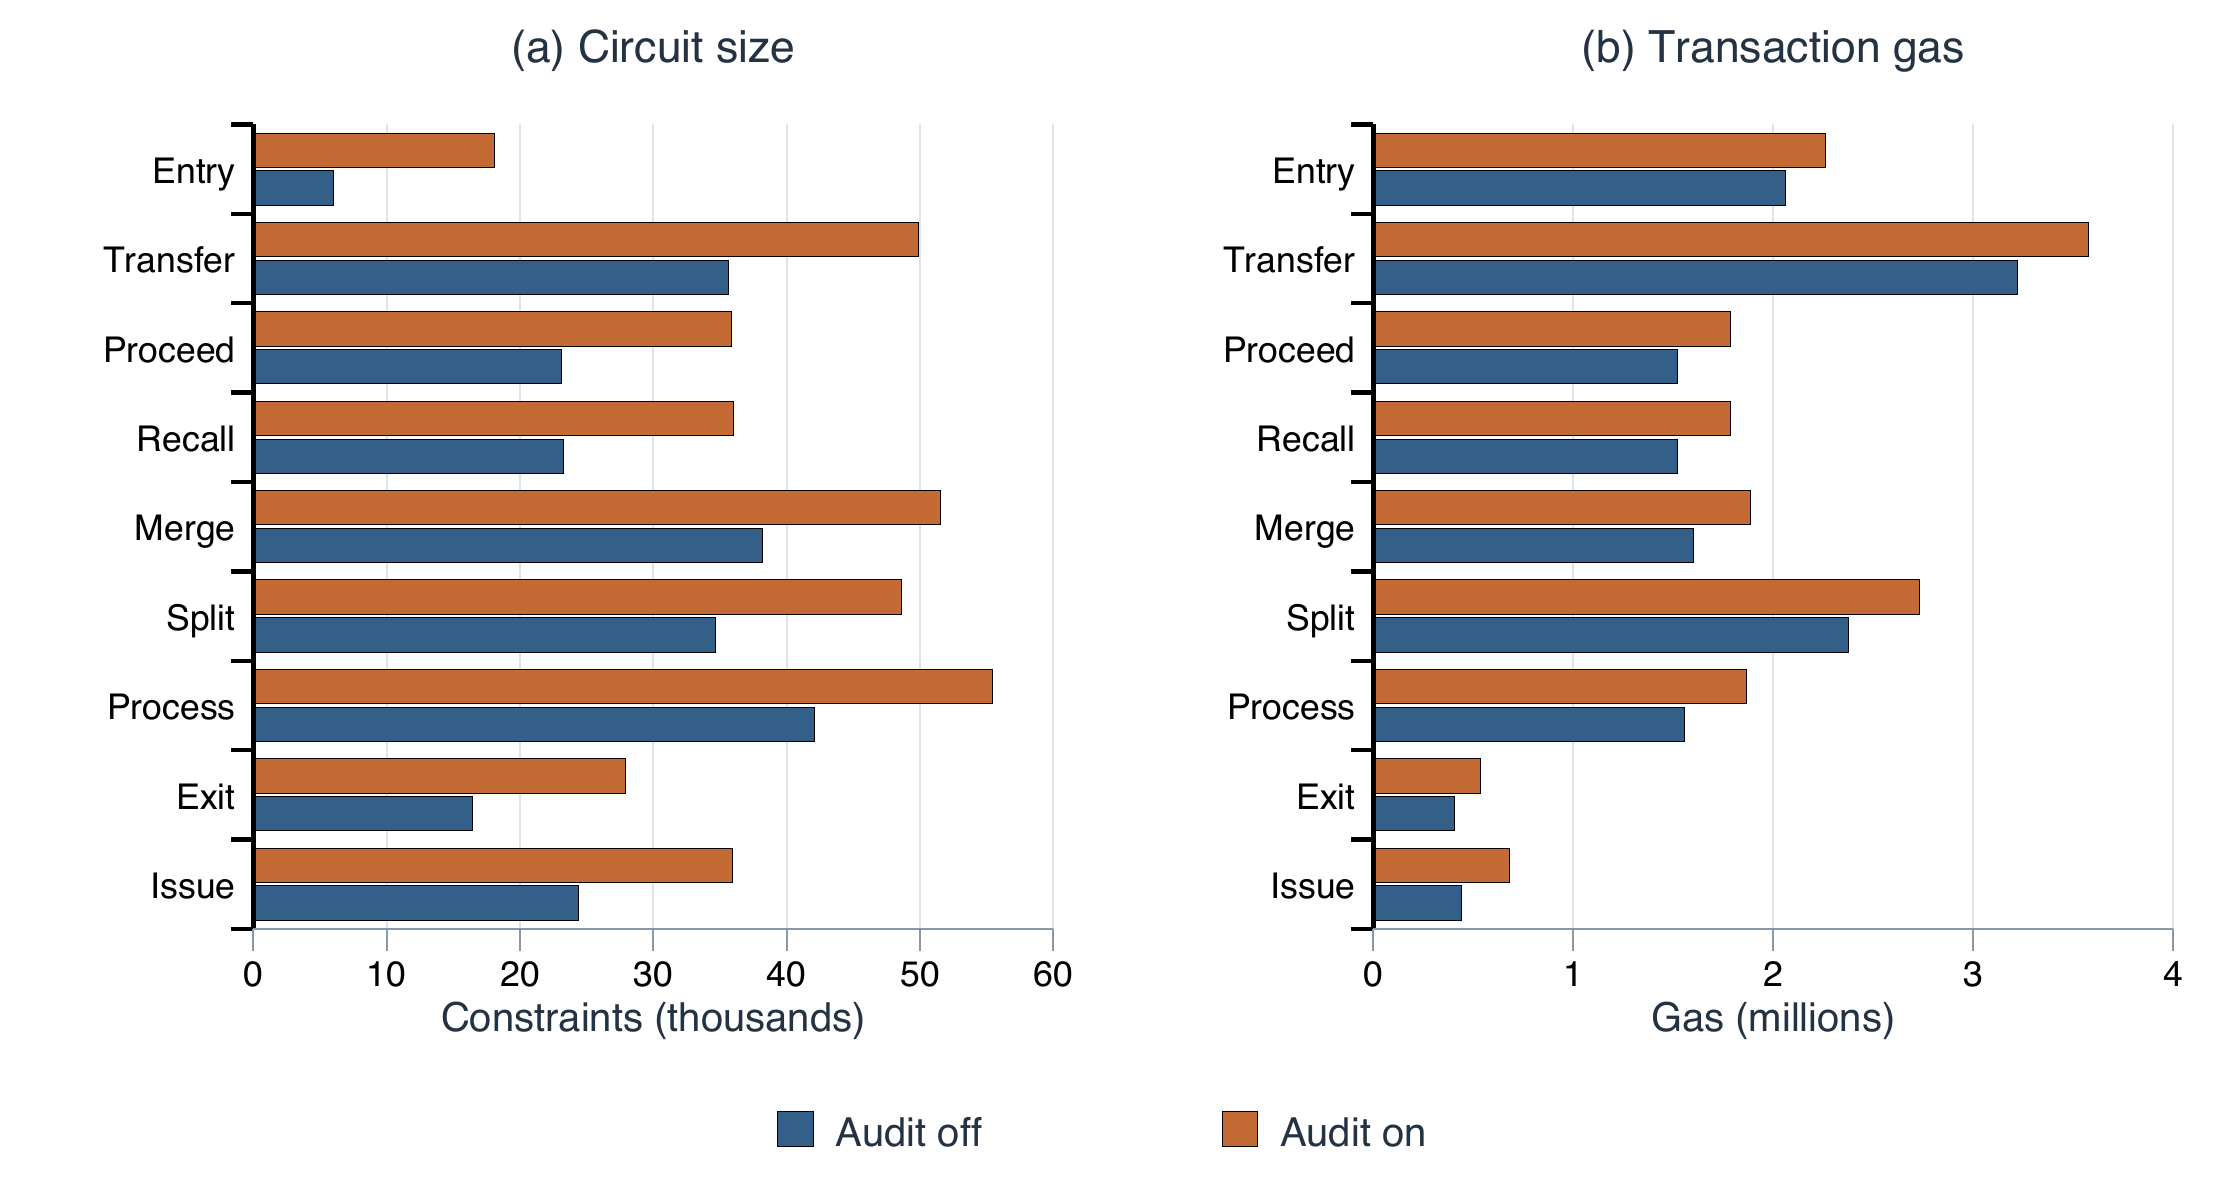
\includegraphics[width=.94\textwidth]{figures/evaluation/audit.png}
\caption{Circuit constraints and transaction gas with and without audit data. The panels use different units.}
\label{fig:eval-audit}
\end{figure*}
\begin{table*}[t]
\centering\small
\caption{Matched audit-off and audit-on costs}
\label{tab:eval-audit}
\begin{tabular*}{\textwidth}{@{\extracolsep{\fill}}lrrrrrr@{}}
\toprule
Event & $C_{\rm off}$ & $C_{\rm on}$ & $\Delta C$ & $G_{\rm off}$ & $G_{\rm on}$ & $\Delta G$ \\ \midrule
Entry & 5,980 & 18,115 & 12,135 & 2,059,123 & 2,258,715 & 199,592 \\
Transfer & 35,645 & 49,883 & 14,238 & 3,221,268 & 3,577,414 & 356,146 \\
Proceed & 23,123 & 35,858 & 12,735 & 1,519,228 & 1,784,082 & 264,854 \\
Recall & 23,252 & 35,987 & 12,735 & 1,520,722 & 1,785,084 & 264,362 \\
Merge & 38,208 & 51,543 & 13,335 & 1,599,289 & 1,888,301 & 289,012 \\
Split & 34,671 & 48,608 & 13,937 & 2,373,759 & 2,730,046 & 356,287 \\
Process & 42,067 & 55,402 & 13,335 & 1,557,348 & 1,866,617 & 309,269 \\
Exit & 16,407 & 27,940 & 11,533 & 403,572 & 534,277 & 130,705 \\
Issue & 24,424 & 35,957 & 11,533 & 438,706 & 678,565 & 239,859 \\
\bottomrule
\end{tabular*}
\par\smallskip\begin{minipage}{\textwidth}\footnotesize $C$: constraints; $G$: gas. Inputs, state, permissions and tree conditions are matched. Differences are on minus off.\end{minipage}
\end{table*}


감사 암호화를 계산할 때에는 타원곡선의 점에 정수를 곱하는
스칼라 곱셈이 사용된다. Transfer의 감사 추가 제약 14,238개 중
이 연산 두 번은
8,611개로 60.48\%를 차지하였다. 나머지는 키·마스크 계산
2,399개, 난수·암호문 검증 1,723개와 출력 소비 식별자 계산
1,505개이다. 감사 추가 gas 356,146 중 감사 기록 저장의
저장 연산 SSTORE는 324,100 gas로 91.00\%이며, 증명 검증 호출 증가분은
4,585 gas, 기타 조회·calldata 증가분은 27,461 gas이다.
따라서 이 거래에서는 두 스칼라 곱셈과 감사 자료 저장이 각각
추가 회로 비용과 추가 원장 비용의 주요 부분을 차지한다.
이 비율은 Transfer의 감사 추가 비용에 대한 분해이다.

\paragraph{추적·동결 규모와 로컬 키 복구.}
추적 규모 $V$는 고유 방문 감사 기록 수, 동결 규모 $F$는 대상
수이다. 같은 Split 시나리오에서 각 작업을 10, 100, 1,000개
규모로 측정하였다. 추적에는 기록 조회·복호화·탐색을, 동결에는
제출 전 상태 검사·대상별 거래 실행·최종 상태 확인을 포함한다.
동결 구현은 대상 하나마다 거래 하나를 제출한다.

\begin{figure*}[t]
\centering
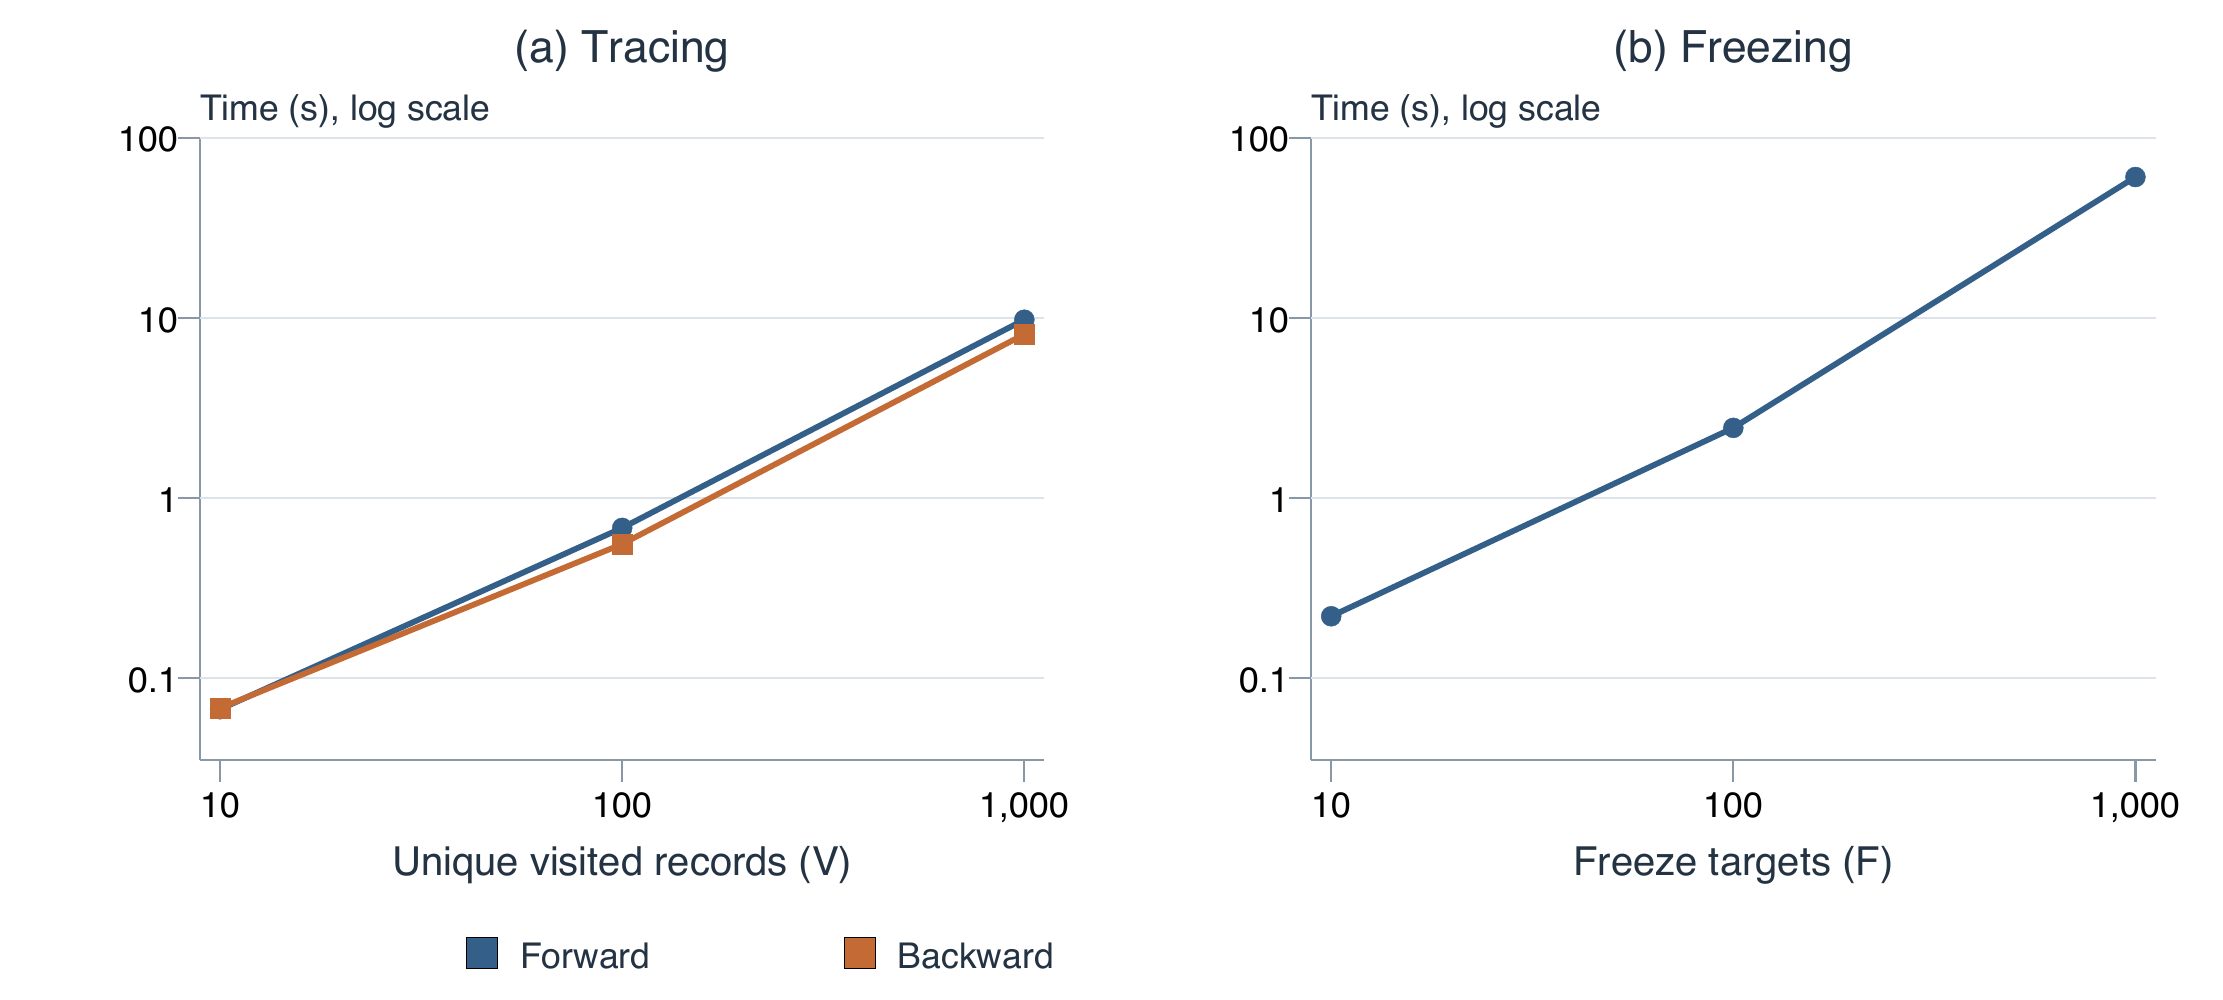
\includegraphics[width=.94\textwidth]{figures/evaluation/tracing-freeze.png}
\caption{Tracing and freezing time. Both panels use logarithmic time axes; $V$ counts visited records and $F$ counts freeze targets. Lines connect measured points.}
\label{fig:eval-trace}
\end{figure*}
\begin{table}[t]
\centering\small
\caption{Time by visited records or freeze targets}
\label{tab:eval-trace}
\begin{tabular*}{\columnwidth}{@{\extracolsep{\fill}}rrrr@{}}
\toprule
$V$ or $F$ & Forward (s) & Backward (s) & Freeze (s) \\ \midrule
10 & 0.067 & 0.068 & 0.220 \\
100 & 0.681 & 0.554 & 2.448 \\
1,000 & 9.760 & 8.102 & 60.540 \\
\bottomrule
\end{tabular*}
\par\smallskip\begin{minipage}{\columnwidth}\footnotesize $V$: unique visited audit records; $F$: freeze targets. The two tasks are measured separately on the Split scenario.\end{minipage}
\end{table}


Table~\ref{tab:eval-trace}에서 기록 1,000개의 선행 추적은
8.102초, 후속 추적은 9.760초이며, 대상 1,000개의 동결은
60.540초이다. 규모가 100에서 1,000으로 증가할 때 시간은
각각 약 14.62배, 14.33배와 24.73배가 되었다.
이 구간에서 동결의 시간 증가가 더 크게 나타났으며,
다만 세 크기만 측정했으므로 더 큰 모든 작업량에서도
어떤 비율로 시간이 늘어날지 일반화할 수는 없다.
활성 회계 증표 하나를 동결 상태로 바꾸는 거래의 gas는
49,434이다. 이는 해당 타입과 상태 전이에 대한 단일 거래의
값으로, 이전 증표나 배치 동결의 비용과 구분한다.
수행 시간 측정과 \ref{sec:audit}절의 전체 완료 조건 검증도
서로 다른 평가 대상이다.

로컬 키 복구는 위원회 공개키와 위원별 공개 조각을 사전에
검증한 뒤, 선택한 $k$개 조각을 검증하고, 조각을 수학적으로 합치는
라그랑주 보간으로 비밀값을 복구한 뒤,
그 결과가 공개키와 맞는지 확인하는 시간을 측정하였다.
전체 위원 수 $n=10$에서 $k$를 2, 3, 5, 7, 10으로 바꾸었다.
공개 자료의 사전 검증, 키 생성·분산 키 생성(DKG), 통신과 승인
대기는 측정 구간에서 제외하였다.

\begin{figure}[t]
\centering
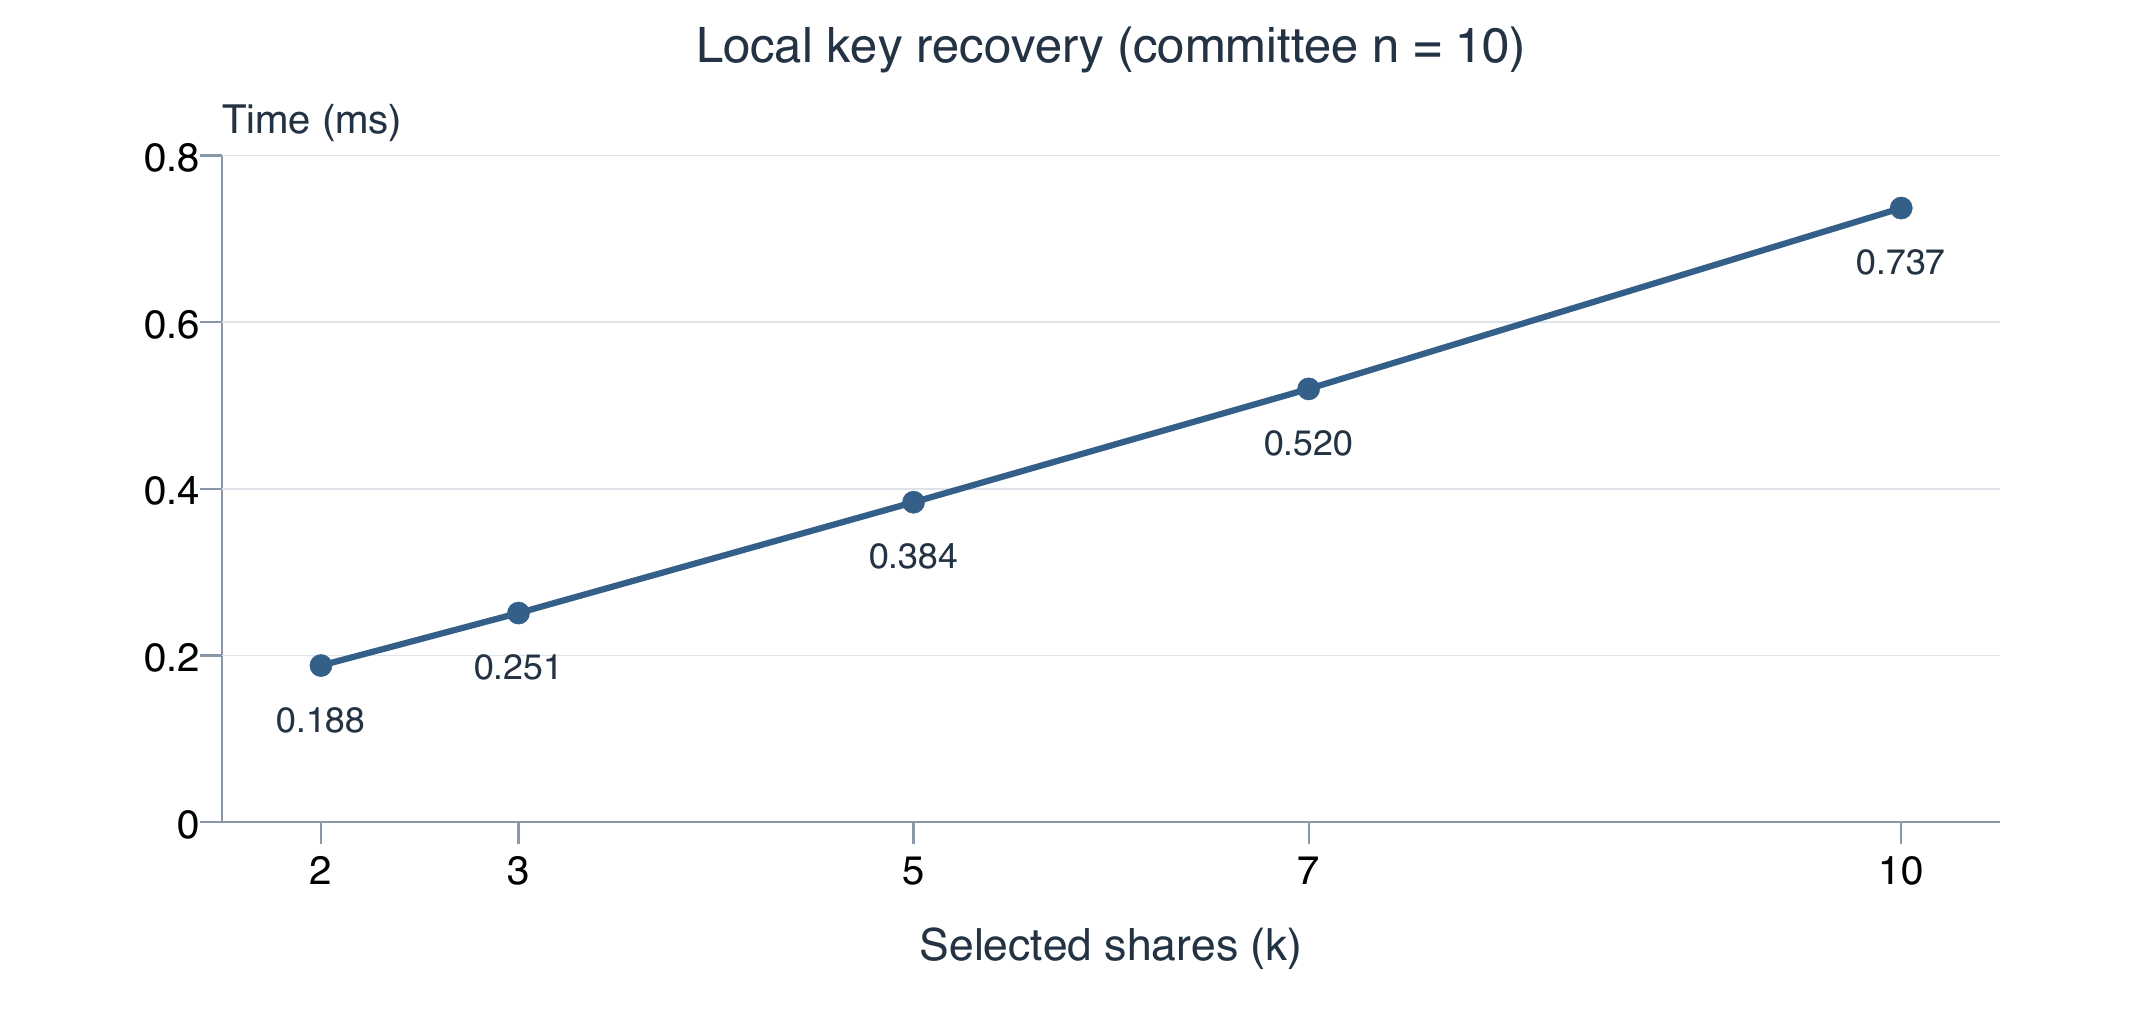
\includegraphics[width=\columnwidth]{figures/evaluation/key.png}
\caption{Local key recovery for $n=10$. Each point is the mean of 1,000 internal recoveries in one timed run after warm-up.}
\label{fig:eval-key}
\end{figure}
\begin{center}
\begin{minipage}{\columnwidth}
\centering\small\captionsetup{hypcap=false}
\captionof{table}{공개 자료 확인 후 감사 비밀키 복원 시간}
\label{tab:eval-key}
\begin{tabular*}{\columnwidth}{@{\extracolsep{\fill}}rrr@{}}
\toprule
전체 위원 수 & 사용 조각 수 & 평균 (ms) \\ \midrule
10 & 2 & 0.188 \\
10 & 3 & 0.251 \\
10 & 5 & 0.384 \\
10 & 7 & 0.520 \\
10 & 10 & 0.737 \\
\bottomrule
\end{tabular*}
\par\smallskip\begin{minipage}{\columnwidth}\footnotesize 준비 실행 뒤 조건마다 한 번 측정하고, 그 안에서 복원 1,000회의 평균을 구했다. 선택한 조각의 검증·결합·복원한 키의 공개키 대조를 포함한다.\end{minipage}
\end{minipage}
\end{center}


Fig.~\ref{fig:eval-key}와 Table~\ref{tab:eval-key}에서 복구 시간은
0.188--0.737\,ms이다. 선택한 조각 집합의 보간식에는 전체 위원
수 $n$이 직접 등장하지 않지만, 이 측정은 $n$을 변화시킨 비교가
아니다. 또한 복구 대상 비밀값과 임계값 $K$의 설정을 현행 두 키
구성에 연결해야 하므로, 이 값을 감사 데이터 키 $SK_B$의
승인·제공 전체 지연으로 해석하지 않는다.

\begin{figure*}[t]
\centering
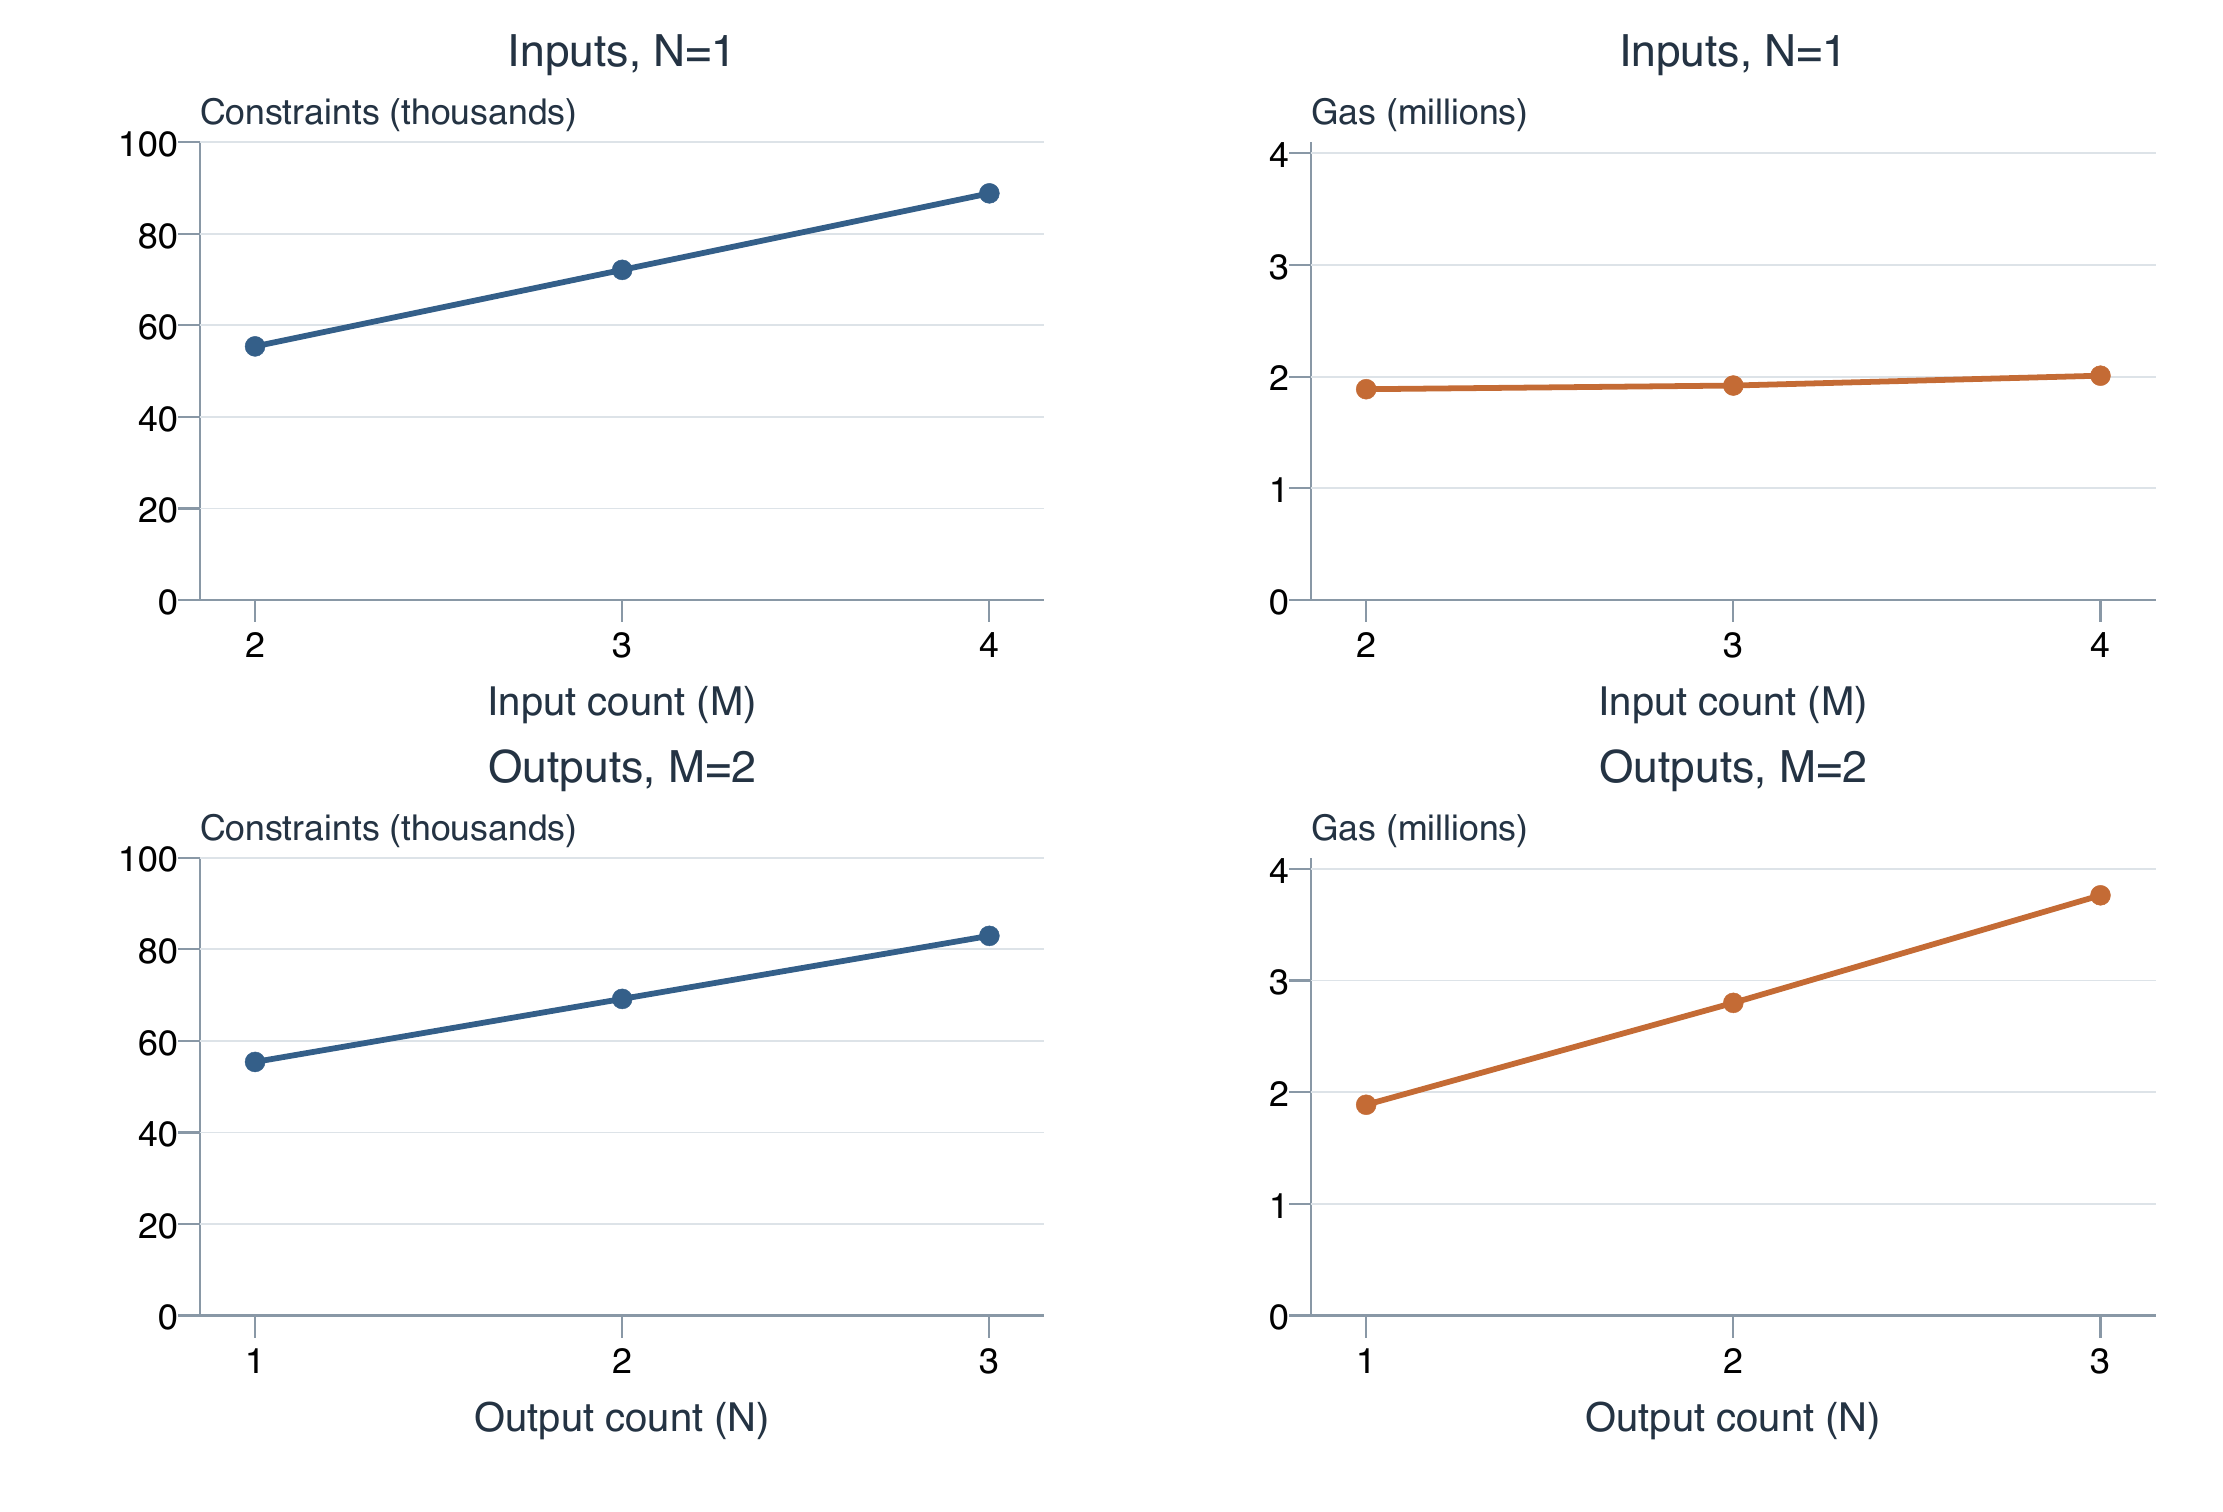
\includegraphics[width=.92\textwidth]{figures/evaluation/process.png}
\caption{Process costs when increasing inputs (top) or outputs (bottom). Matching metrics use the same vertical range; lines connect measured points.}
\label{fig:eval-process}
\end{figure*}

\paragraph{전달 방식과 공정 입출력의 영향.}
직접 전달은 송신 거래에서 수신자 회계 증표를 생성하고,
이전 증표 방식은 Transfer로 미해결 이전을 만든 뒤 Proceed로
수령을 완료한다. Table~\ref{tab:eval-transfer}은 직접 전달,
SharedSecret 변형과 정상 수령·회수 경로를 구분한다.

\begin{center}
\begin{minipage}{\columnwidth}
\centering\small\captionsetup{hypcap=false}
\captionof{table}{원료 전달 방식별 비용과 기능}
\label{tab:eval-transfer}
\begin{tabularx}{\columnwidth}{@{}p{20mm}rY@{}}
\toprule
방식 & gas & 기능 차이 \\ \midrule
직접 전달 & 2,366,228 & 감사 자료와 송신자 회수 기능 없음 \\
SharedSecret & 2,724,242 & 감사 자료 있음; 송신자가 후속 소비 식별 가능 \\
T $\to$ Proceed & 5,361,496 & 인수 전 회수 가능; 인수 뒤 소비는 직접 식별 불가 \\
T $\to$ Recall & 5,362,498 & 송신자가 인수 전에 회수 \\
\bottomrule
\end{tabularx}
\par\smallskip\begin{minipage}{\columnwidth}\footnotesize
T는 Transfer다. 직접 전달에는 감사 자료가 없고 다른 방식에는 있다.
기능 열은 설계상의 차이를, gas 열은 측정한 거래 비용을 나타낸다.
T $\to$ Proceed의 gas는 두 거래의 합이다. T $\to$ Recall은
보고된 경로 총합이며 두 거래의 합과 일치한다.
\end{minipage}
\end{minipage}
\end{center}


정상 수령의 합산 비용은
$3{,}577{,}414+1{,}784{,}082=5{,}361{,}496$ gas이다.
회수 경로의 5,362,498 gas는 Transfer와 Recall의 합이다.
정상 수령 합산값은 감사 없는 직접 전달의 약 2.266배다.
그러나 두 방식은 감사 기능의 유무도 다르고 거래 단계 수도 다르다.
따라서 이전 증표를 사용했기 때문에만 비용이 그만큼
늘었다고 해석할 수는 없다. 합산값은 연속 실행의 직접
측정값과도 구분한다.

이전 증표는 미해결 상태에서 기한·권한 조건을 만족하면 회수할 수
있으며, Proceed와 Recall이 같은 $rvnf$를 소비하므로 먼저
수락된 경로만 성공한다.
비교용 SharedSecret 직접 전달은 공유값 $o_{\rm shared}$를 이용한
$nf_{\rm shared}=H(cm,o_{\rm shared})$로 소비 식별자 계산 방식을 바꾼다.
송신자도 $cm,o_{\rm shared}$를 알면 수신자 회계 증표의 소비 거래를 식별할 수
있으나 소비 권한을 얻는 것은 아니다.
이 변형의 2,724,242 gas는 감사 없는 직접 전달보다
358,014 gas 크다. 감사 자료와 식별자 계산 방식이 함께 달라
감사 기능만의 비용으로 해석하지 않는다.

이전 증표의 공유 개방값으로 송신자가 계산하는 것은 $rvnf$이다.
인수 후 수신자 회계 증표의 $nf$는 수신자 소유 비밀에 의존하므로
그 개방값만으로 직접 계산할 수 없다. 이는 공개 시각·메타데이터를
이용한 모든 추론을 배제하는 성질은 아니다.
감사자는 Transfer에서 $rvnf$를 복원하여 Proceed를 찾고,
그 기록에서 수신자 회계 증표의 미래 $nf$를 복원한다.
잔여 회계 증표도 별도의 미래 식별자를 통해 추적한다.

공정 규모는 출력 $N=1$에서 입력 $M$을 2, 3, 4로,
입력 $M=2$에서 출력 $N$을 1, 2, 3으로 바꾸어 평가하였다.
입력 상태 합 $(320,30,231)$과 출력 상태 합 $(300,30,261)$을
고정하였다. 이 조건은 시제품의 세 상태 성분에 대한 것으로
모든 산업 공정을 대표하지 않는다.

\begin{table}[t]
\centering\small
\caption{Process cost by input and output count}
\label{tab:eval-process}
\begin{tabular*}{\columnwidth}{@{\extracolsep{\fill}}lrrrr@{}}
\toprule
Sweep & $M$ & $N$ & Constraints & Gas \\ \midrule
Inputs & 2 & 1 & 55,402 & 1,887,935 \\
Inputs & 3 & 1 & 72,116 & 1,920,611 \\
Inputs & 4 & 1 & 88,832 & 2,009,039 \\
Outputs & 2 & 1 & 55,402 & 1,887,935 \\
Outputs & 2 & 2 & 69,172 & 2,800,596 \\
Outputs & 2 & 3 & 82,944 & 3,763,779 \\
\bottomrule
\end{tabular*}
\par\smallskip\begin{minipage}{\columnwidth}\footnotesize Input sum $(320,30,231)$ and output sum $(300,30,261)$ are fixed. The $2\to1$ baseline differs by 21,318 gas from Table~\ref{tab:eval-events}; the cause is unresolved.\end{minipage}
\end{table}


Table~\ref{tab:eval-process}에서 입력을 2개에서 4개로 늘리면
제약 수는 60.34\%, gas는 6.41\% 증가하였다. 출력을 1개에서
3개로 늘리면 각각 49.71\%와 99.36\% 증가하였다.
이 구간에서는 출력 증가가 입력 증가보다 gas에 더 큰 변화를
동반하였다. 입력이 늘면 기존 기록을 검사하는 일이 추가되고,
출력이 늘면 새 기록을 등록하는 일이 추가된다.
관측값은 이 차이와 부합하지만, 어느 연산이 얼마를 차지하는지는
비용을 더 나누어 측정해야 알 수 있다.
이 실험의 $M=2,N=1$ gas는 1,887,935로 기본 거래의
1,866,617과 21,318 차이가 난다. 증가율은 공정 규모 실험
안의 기준값으로 계산하며, 두 실행의 차이는 미확인으로 남긴다.

\subsection{기존 연구와의 비교}

\begin{table}[t]
\centering\small
\caption{Published and measured transaction gas}
\label{tab:eval-published}
\begin{tabularx}{\columnwidth}{@{}>{\raggedright\arraybackslash}p{24mm}rY@{}}
\toprule
System or path & Gas & Scope \\ \midrule
Azeroth zkTransfer~\cite{jeong-azeroth-2023} & 1,555,957 & Published; change in ENA \\
Direct baseline & 2,366,228 & No audit; change Note \\
SharedSecret direct & 2,724,242 & Audit; shared spend identifier \\
zkDPP Transfer & 3,577,414 & Audit; Voucher and change Note \\
zkDPP Transfer $\to$ Proceed & 5,361,496 & Normal receipt; two-event sum \\
\bottomrule
\end{tabularx}
\par\smallskip\begin{minipage}{\columnwidth}\footnotesize Azeroth: Groth16, MiMC7, depth 32. Remaining rows: this evaluation. Different settings and functionality preclude an efficiency ranking.\end{minipage}
\end{table}


Table~\ref{tab:related}의 기능 비교를 바탕으로,
평가에서는 추적·차단의 작업 단위와 거래 비용을 비교한다.
Sahai 등의 공급망 전이와 Babel 등의 자격증명·토큰 연결은
응용 측면의 기준선이며, GGM의 후속 출력 추적, Azeroth의
거래 결합 감사 정보와 CAP의 정책별 열람·동결은 감사·집행의
선행 구성이다. zkDPP의 기능 검증은 이를 회계 전이,
제품 주장·종료의 구분, 미소비 회계 증표·미해결 이전 증표의
차단으로 연결한 대표 경로를 확인한다. 같은 응용 관계와 신뢰
조건을 갖는 구성보다 우수하다는 결론은 이 검증에서 도출하지 않는다.

Azeroth는 Groth16, MiMC7, 깊이 32의 설정에서
zkTransfer의 비용을 1,555,957 gas로 보고한다~\cite{jeong-azeroth-2023}.
Table~\ref{tab:eval-published}은 이 값과 본 평가의 전달 비용을
작업 범위와 함께 제시한다. Azeroth는 암호화 계정(ENA)과
머클 노트를 함께 사용하여 잔여 금액을 ENA에 반영하고,
본 평가의 직접 전달 기준선은 잔여분을 새 회계 증표로 등록한다.
증명계·검증기·해시·원장 조건도 같지 않다.
이 표는 각 전달 방식에서 무엇을 하나의 작업으로 측정했는지
보여 주며, gas 차이를 잔여분 처리 방식 하나의 효과로 분리하지는 못한다.
자체 직접 전달은 Azeroth를 같은 환경에서 재현한 결과가 아니다.

Sahai의 Hyperledger Fabric 구현은 EVM gas와 다른 지표를
사용한다~\cite{sahai-supply-chain-2020}.
Babel 등의 측정은 분산 원장을 사용하지 않는 운영자 원장을
대상으로 하므로 그 연산 시간을 거래 영수증 확인까지 포함한
E2E와 직접 비교할 수 없다~\cite{babel-hicss-2025}.
CAP의 동결도 레코드의 소비·재발행으로 이루어져 현재 상태를
변경하는 zkDPP와 작업 구성이 다르다~\cite{espresso-cap-spec-2022}.
따라서 본 평가는 대표 기능의 연결과 기능별 비용·규모 변화를
제시하며, 외부 시스템과의 효율성 순위를 정하지 않는다.
% Flush evaluation floats; restore the full text height after double-column floats.
\clearpage
\makeatletter
\global\@colht\textheight
\global\@colroom\textheight
\global\vsize\textheight
\makeatother
